\mysubsection{Fabian Gärtner}{Personenerkennung mittels Microsoft Kinect}

Zur Erkennung von Personen auf dem Spielfeld mittels Microsoft Kinect konnten keine Standardfunktionen verwendet werden, da das Kinect-SDK den Einsatz der Kinect aus der Vogelperspektive nicht vorsieht. Stattdessen muss das von der Kinect aufgenommene Tiefenbild mittels gesonderter Bildverarbeitung auf Personen bzw. auf Objektkonturen untersucht werden. In BlinkenTiles sind dafür die drei Klassen \enquote{KinectManager}, \enquote{BlobDetection} und \enquote{BlobDetectionThread} zuständig. Erstere fragt unter Anwendung des Kinect-SDKs das Tiefenbild (30 Bilder pro Sekunde mit einer Auflösung von 512 x 424 Pixel) und -- bei Bedarf -- das Farbbild (15 Bilder pro Sekunde mit einer Auflösung von 1920 x 1080 Pixel) der Kinect ab. Das Tiefenbild ist dabei ein zweidimensionales Array des Datentyps \emph{short}, das mit Werten zwischen 0 und 8000 die pro Pixel gemessene Entfernung in Millimeter angibt. Da sich das Farbbild vom Tiefenbild in Auflösung und Bildwinkel unterscheidet, müssen die Werte des Farbbildes, um beide Bilder übereinander legen zu können, mittels einer vom Kinect-SDK bereitgestellten Mapping-Funktion umgerechnet werden. Auch dies übernimmt die Klasse. Des Weiteren besteht hier auch die Möglichkeit Tiefenbilder in Form von Dateien abzuspeichern und für den Fall, dass die Kinect nicht angeschlossen ist, als Testdaten zu verwenden.

Die Klasse \enquote{BlobDetection} ist hauptsächlich für die Verwaltung der grafischen Benutzeroberfläche und der beiden anderen Klassen zuständig. Die grafische Benutzeroberfläche für die Bildverarbeitung, wie sie in Abbildung X dargestellt ist, nimmt die linke Hälfte der gesamten GUI von BlinkenTiles ein und erstreckt sich damit über einen Monitor. Dies ist notwendig, da viele verschiedene Einstellungen möglichst genau vorgenommen werden müssen, um eine optimale Personenerkennung zu gewährleisten. Es ist deshalb möglich, die Ansicht zwischen verschiedenen Vearbeitungsschritten zu wechseln und diese zu über Slider zu konfigurieren. Ebenso kann ein Raster über dem Tiefenbild angezeigt werden, bei dem alle aktivieren Felder, also alle Felder auf denen Personen erkannt wurden, farbig markiert sind. Um dieses Raster dem vom Beamer erzeugten Spielfeld anzupassen kann ebenso eine Überlagerung von Farb- und Tiefenbild angezeigt werden, die dann eine Ausrichtung des Rasters mittels der Slider erlaubt. Bla bla bla bla bla bla bla bla bla bla Bla bla bla bla bla bla bla bla bla bla

Die eigentliche Bildverarbeitung findet in der Klasse \enquote{BlobDetectionThread} statt und wird zur Laufzeit in einem eigenen Thread ausgeführt. Dies war anfangs notwendig, da die Bildverarbeitung zu einer niedrigen Bildrate in der Hauptanwendung führte. Dieser Prozess konnte im Verlauf der Entwicklung aber stetig optimiert werden, sodass die Bildverarbeitung auf eine Dauer von lediglich 12ms pro Tiefenbild reduziert werden konnte. Mit etwas mehr als 80 Bildern pro Sekunde liegt die Bildverarbeitung weit über der Bildrate der Kinect mit rund 30 Bildern pro Sekunde. Damit ist eine Personenerkennung ohne Verzögerung und in Echtzeit möglich. Die Auslagerung in einen eigenen Thread wurde aber beibehalten, so dass die Arbeitslast gleichmäßig auf mehrere CPU-Kerne verteilt wird und auch mögliche Hänger der Kinect keine Auswirkung auf die Hauptanwendung haben.

Hauptsächlich für die Bildverarbeitung verwendet wird die kostenfreie Open-Source-Bibliothek OpenCV, die über den C-Sharp-Wrapper EmguCV angesteuert wird. OpenCV erlaubt die Anwendung von Algorithmen und grundlegenden mathematischen Operationen auf Matrizen und Bilder. Konkret wird bei BlinkenTiles zunächst das als short-Array vorliegende Bild gefiltert und normalisiert. Die Filterung arbeitet anhand der vom Nutzer eingestellten Werte für minimale und maximale Tiefe. Alle werte über und alle Werte unter den Vorgaben werden auf 0 gesetzt, sodass diese die Erkennung nicht weiter stören. Ein Anwendungsfall hierfür ist der von der Kinect erkannte Boden. Reflektiert der Boden zu stark würde die Kinect ihn als ein großer Blob erkennen. Durch die Filterung können nun die Werte herausgefiltert werden, die dem Abstand zum Boden entsprechen (+/- Toleranz), so dass nur noch Objekte bzw. Personen erkannt werden, die näher an der Kamera sind als der Boden. Die Normalisierung hilft dann den Kontrast des Tiefenbildes zu erhöhen und so die dann folgende Binarisierung des Bildes zu optimieren. Auf das binarisierte Bild wird dann die Konturerkennung von OpenCV angewendet, die Objekte ab einer bestimmten Größe erkennt und ein entsprechendes Bounding-Rectangle zurückliefert. Dieses Rechteck kann dann mit den Feldern der Matrix abgeglichen werden und bei Schnitten zwischen Bounding-Rectangle und einem Feld das Feld aktiviert werden. Zwischendurch werden regelmäßig für den Präsentationsbildschirm die einzelnen Schritte als Bilder herausgespeichert.

Am Tag der Medien zeigte sich, dass die Tische, auf denen u.\,a. die LED-Scheinwerfer standen, aufgrund ihrer hellen Oberfläche nicht aus dem Tiefenbild herausgefiltert werden konnten. Dies führte dazu, dass Personen, die auf einem der Felder in der Nähe der Tische standen, zusammen mit den Tischen als ein großes Objekt erkannt und dadurch gelegentlich zu viele Felder gleichzeitig aktiviert wurden. Beheben ließe sich das Problem, indem das Tiefenbild vor der Verarbeitung auf den relevanten Bereich zugeschnitten wird. Auch hierfür könnten entsprechende Regler in die GUI integriert werden, sodass der Zuschnitt manuell und je nach Bedarf eingestellt werden kann.

Ein größeres Problem ist die Perspektive, vor allem dann, wenn die Kinect nicht mittig über dem Spielfeld hängt. So funktioniert die Erkennung von Personen, die sich direkt unter der Kinect befinden zwar tadellos, je weiter eine Person aber von der Kinect entfernt ist, desto mehr Felder deckt sie aufgrund der schrägen Aufsicht gleichzeitig ab. Eine kurzfristige Lösung am Tag der Medien war es, die Felder in der Anwendung größer einzustellen als sie eigentlich sind. Des Weiteren wird bereits nicht das ganze Feld auf Überdeckung geprüft, sondern lediglich ein kleinerer (ebenfalls einstellbarer) Bereich in der Mitte der Felder. Dadurch verringert sich das Problem der schrägen Aufsicht und es werden seltener mehrere Felder gleichzeitig aktiviert. Um das Problem aber besser zu lösen wäre entweder eine zweite Kinect oder eine korrekte Berechnung und eine unsymmetrische Rasterung notwendig. Bspw. könnte zu den Rändern hin die Tiefenfilterung angepasst werden, sodass in diesen Bereichen nur noch die Beine von Personen relevant sind für die Überdeckung, nicht aber der Kopf, der möglicherweise ein anderes Felder überdeckt.


\newpage

\begin{figure}[htbp] 
  \centering
     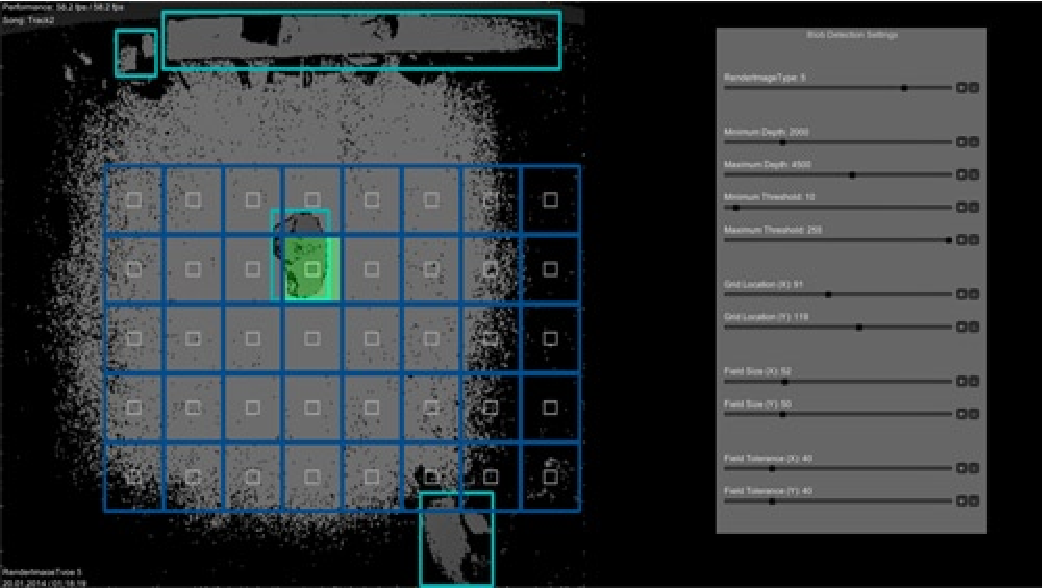
\includegraphics[width=0.9\textwidth]{images/Blob}
  \caption{Schneiden der Spuren in Ableton Live}
  \label{fig:audio1}
\end{figure}